\chapter{Ongoing and Proposed Research}

%\chapter{Event Detection based on Information Absenteeism}
%Information Absenteeism Detection on Social Graphs
% if you want to define paper specific  macros
% then put everthing between begingroup and endgroup
\begingroup
\newcommand{\score}{S}
\newcommand{\myalgo}{CoolAlgo}


%\begin{abstract}
%Event detection in online social media has primarily focused on identifying
%abnormal spikes, or bursts, in activity. However, disruptive events such as socio-economic disasters, civil unrest, and even power outages, often result in abnormal troughs involving group absenteeism of activity. We present the first study, to our knowledge, that models absenteeism and uses detected absenteeism as a basis for event detection in location based social networks (LBSN) such as Twitter. Our framework addresses the challenges of (i) early detection of absenteeism, (ii) identifying the point of origin, and (iii) identifying groups or communities underlying the absenteeism. Our approach uses the formalism of graph wavelets to represent the spatiotemporal structure and user activity in a LSBN. This formalism affords multiscale analysis, enabling us to detect anomalous behavior at different graph resolutions, which in turn allows identification of event location and anomalous groups underlying the network. We introduce a systematic two-pass detection method using graph wavelets to detect group absenteeism and then check if there is a subsequent activity spike. The effectiveness of our approach is highlighted with three case studies involving Twitter activity over Latin American countries.
%\end{abstract}

\section{Event Detection from Group Absenteeism}


Social microblogs such as Twitter and Weibo are experiencing explosive growth, with billions of users globally sharing their daily status updates online.
For example, Twitter has more than 255 million average monthly active users (78\% from mobile) as of March 31, 2014, and an estimated increase of 25\% per year\footnote{http://solomozone.com/tag/revenues/}.
Various studies have shown that Twitter is viable as a social ``sensor'', and holds great promise for detecting and forecasting significant societal events~\cite{bugel2013multilingual,sakaki2010earthquake}.
In recent years, a significant body of research~\cite{aggarwal2012event,hong2012discovering,lappas2009burstiness,lappas2012spatiotemporal,sakaki2010earthquake,sayyadi2009event,watanabe2011jasmine,weng2011event,yin2011geographical} has focused on modeling bursts and increases of user activity in social media.

However, real world events are not only correlated with burst signals, but can also exhibit unusually low levels of activity in social networks.
As shown in Figure 1, a protest in the city of Natal, Brazil began at 5:00 PM (local time) at the Museum of the Republic, with people gradually joining the demonstration. %\footnote{http://www.jb.com.br/pais/noticias/2013/06/17/manifestantes-invadem-cobertura-do-congresso-nacional-em-brasilia/}.
On Twitter, there was an uncharacteristic lull in activity or {\it group absenteeism} behavior from 6:00 PM---8:00 PM on the same day.
%Another example comes from December 24, 2013, southern Brazil experienced widespread flash floods. According to news sources, more than 50,000 people were forced to flee their homes in Minas Gerais and Espirito Santo, in the southern states of Brazil. Immediately following the floods, Twitter activity in this region dropped by 51\%, and reached its lowest point that evening.
%Other examples of \textit{group absenteeism} that we observed from Latin American Twitter activity include bus strikes in Brazil on May 21, 2014, the Iquique earthquake in Chile on April 1, 2014, and a major power supply disruption in Argentina on December 30, 2013.

\begin{figure}[t]
\centering
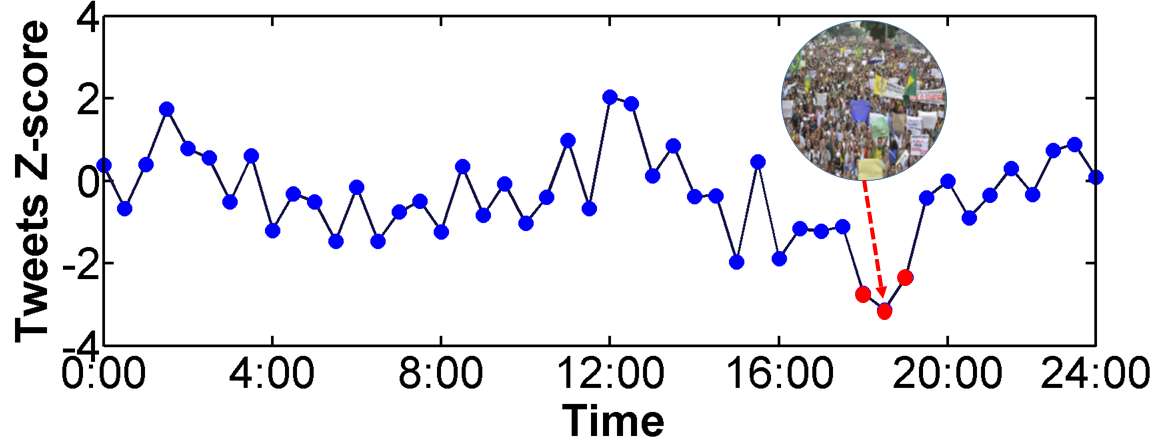
\includegraphics[height=1.1in]{figures/Natal_example1.png}
\caption{Detected group absenteeism in Natal, Brazil beginning at 6:00 PM on June 17, 2013. This absenteeism event coincides with a large protest that happened in the region.}
\vspace{-1em}
\label{fig:natal-protest}
\end{figure}

Investigating this phenomenon of unusually calm behavior online holds enormous potential for understanding localized, disruptive societal events. One recent research work~\cite{chi2015ghost} detects vacant housing areas in China using using Baidu positioning data, which is a practical application of absenteeism study. In this paper we focus on absenteeism based event detection, and introduce this important topic as a key data mining task for social media analytics.
An \textit{absenteeism} event in social networks can be defined as an event which is characterized by a significant lull in activity such as a sudden, sharp decrease of Twitter volume within a short period of time (and which  often precedes a major burst in re-activity).
This paper presents the first study to systematically investigate group absenteeism in LBSNs.
Using graph wavelet techniques, we pose this problem as one of group anomaly detection.
%To appropriately incorporate absenteeism concepts into our detection approach, we must first address the following questions:
%\begin{itemize}
%\item What scale should we select to model the absenteeism groups? %Which node should be the central point?
%
%\item What is the most efficient approach to select absenteeism groups that are spatially and temporally localized?
%
%\item How do we model an absenteeism signal for event detection? Even though we have clear examples of real world events which can explain the observed absenteeism, not all absenteeism occurrences can be associated with underlying events. Therefore we must be able to differentiate absenteeism from noisy signals for event detection.
%\end{itemize}

Graph wavelets display two outstanding advantages to study the above
questions: scalability and low computational complexity.
In this scenario, the data objects are embedded in a general graph as vertices.
By employing wavelet transforms on the graph, we can construct a wavelet function with a graph structure, and we are able to select absenteeism groups at different scales.
Lastly, we propose a two-pass group anomaly detection method that first detects absenteeism, and then checks if there is a subsequent burst in activity within a specific time period.
By comparing correlations between the wavelet coefficients of both of these groups, we are able to relate observed absenteeism to a possible real world event.


Our contributions are:
\begin{itemize}
\item We propose the method to modeling group absenteeism as a basis for event detection.
%Even though burst has been extensively discussed in previous work, however, the absenteeism has different patterns and plays an irreplaceable role in event detection.
\item We incorporate graph wavelets as a mechanism to detect the most anomalous subgraphs at different scales. We demonstrate how this is a powerful technique for social media analytics.
\item We propose a novel two-pass event detection method that uses correlation scores between the group depicting \textit{absenteeism} and the group demonstrating increased activity to probabilistically determine the likelihood of an event.
\end{itemize}

%The rest of the paper is organized as follows. Section~\ref{sec:related} reviews related work and existing methodologies and Section~\ref{sec:preliminaries} formalizes the research problem. In Section~\ref{sec:algorithm}, we first discuss the graph wavelet formalism for group absenteeism detection, and subsequently demonstrate how it can be used for two-pass event detection. Section~\ref{sec:experiment} presents extensive experiments for event detection, and the paper concludes with a summary of the research in Section~\ref{sec:conclusion}.


\subsection{Problem Statement}
\label{sec:problemformulation}
We focus on the problem of event detection from online social networks, based on the absenteeism behavior observed in user activity in geographically proximal communities or group of cities.
We define this problem as following: \emph{given a graph and \textit{absenteeism score} vector, $\mathbf{G}(V,E,W;f^t)$ at time interval $t$, select a subset $\Sigma \subseteq V$, such that
\vspace{-0.5em}
\begin{eqnarray}
 \label{eq: problem}
    \Sigma=\underset{P\subseteq V, P \mbox{ is compact}}{\arg\min}\ \ \sum_{v_k\in P} {f(k)}
\end{eqnarray} }

A general solution to this problem is using a combinatorial optimization technique, where by defining a constrained objective function over a network one can identify subset of vertices which maximize the corresponding function~\cite{rozenshtein2014event}. Therefore, Equation~\ref{eq: problem} can be modified as:
\vspace{-0.5em}
\begin{eqnarray}
 \label{eq: problem_conventional}
    \Sigma=\underset{P\subseteq V}{\arg\min}\ \ \sum_{v_k\in P} {f(k)}+\lambda \mu(P)
\end{eqnarray}
, where $\mu(P)$ is the compactness penalty function of $P$ (e.g., the sum of distances among
all pairs of the vertices in $P$~\cite{rozenshtein2014event}), and $\lambda$ is the regularization parameter.
Such methods suffer from the following issues:
\begin{enumerate}
\item To define and measure the compactness of subset $P\subseteq V$ is challenging, considering the exponential varieties of complex graphs.
\item To determine a suitable regularization parameter $\lambda$ in the objective function is ambiguous, because simply combining multiple physically different concepts in the objective function makes the optima sensitive to $\lambda$.
\item To solve this objective function is often a \textbf{NP-hard} problem, which makes it unpractical in many real world applications. Sometimes, even the approximate solutions are of high computation complexity, if there are any.
\end{enumerate}

In contrast, our approach proposes a novel, absenteeism based events detection algorithm in social networks using spectral graph wavelet theory.
The graph wavelets focus on the intrinsic geometric structure of the graph by transversing each vertex $v_i\in V$, and mining the topological information of both local and globally centered vertices supports the ability to conduct a multiscale analysis.
In addition, the graph wavelet approach does not introduce any ``subjective'' objective functions or other compactness concepts, and thus provides a fair and low computational method in terms of complexity for identifying abnormal group behavior in a wide variety of application scenarios.

\subsection{Graph Wavelet}
Classic wavelet is called mathematical microscope since it is capable of showing signal abnormality with different scales. In the case of complex networks, graph wavelets render the graph with good localization properties both in frequency and vertex (i.e. spatial) domains. Their scaling property allows us to zoom in/out of the underlying structure of the graph.

It is useful to analyze $f$ by taking into account the intrinsic geometric structure of the graph $\mathbf{G}$. In order to identify and exploit structure of  $f\in \mathbb{R}^N$, the spectral graph $\sigma({\mathcal{L}}):=\{\chi_l\}_{l=0}^{N-1}$ can be used as a dictionary of atoms~\cite{shuman_ACHA_2013}. Thus, $f$ can be decomposed as a linear combination of $\{\chi_l\}_{l=0}^{N-1}$ as
\vspace{-0.5em}
\begin{equation}
\label{eq:graph_fourier}
f(n)= \sum\limits_{l=0}^{N-1}\hat{f}(l)\chi_l(n)
\end{equation}
\vspace{-0.5em}
, where
\vspace{-0.5em}
\begin{equation}
\label{eq:graph_fourier1}
\hat{f}(l):= \sum\limits_{n=0}^{N-1}\chi^*_l(n)f(n)
\end{equation}
$\chi_l$ is called the Fourier frequency of $f(n)$ based on the graph $\mathbf{G}$, and $\hat{f}(l)$ is the corresponding Fourier coefficient.
Equation~\ref{eq:graph_fourier1} and Equation~\ref{eq:graph_fourier} are called Fourier transform and inverse Fourier transform, respectively.
Equation~\ref{eq:graph_fourier1} gives a clear representation of the Fourier components in $f(n)$.
However, information concerning the vertex-location can not be identified from the Fourier transform. To address this issue, Hammond et al.~\cite{hammond2011wavelets} proposed constructing wavelet transforms of functions over the vertices using weighted graphs, described in the following steps:

\begin{enumerate}
\item Define a continuous generating kernel functions $g(x)$ on $\mathbb{R}^+$;
\item Then, select a central vertex $v_a \in {V}$ and scale $s$, set the frequency coefficients as $g(s\lambda_l)\chi^*_l(a)$ for each frequency component $\chi_l$;
\item Finally, sum up all those frequency components $\chi_l$.
\end{enumerate}
In this way, the graph wavelet at central vertex $v_a$ is constructed as:
\vspace{-0.5em}
\begin{equation}
\label{eq:graphwaveletdefinition}
\psi_{s,a}(n) = \sum\limits_{l=0}^{N-1}g(s\lambda_l)\chi_l^*(a)\chi_l(n)
\end{equation}
After setting up the graph wavelet, the wavelet coefficients for $f$ can be defined as
\vspace{-0.5em}
\begin{equation}
\label{eq:graph_graphwavelet}
W_f(s,a)=<\psi_{s,a}, f>=\sum\limits_{l=0}^{N-1}g(s\lambda_l)\hat{f}(a)\chi_l(n)
\end{equation}



\subsection{Two-pass Event Detection Model}

We intend to propose a two-pass absenteeism based event detection algorithm. The underlying rationale of this algorithm is based on the following concepts.
\begin{enumerate}
\item As discussed above, distribution of $f$ can be well reconstructed by the $J$ scaling and $NJ$ wavelet coefficients. Each of those normalized wavelet coefficients $W'_f(s,a)$ represents a distribution pattern of $f$ on $\mathbf{G}$.
It is equivalent to saying that $\psi_{s,a}$ represents a special distribution pattern, which shares a large and uniform value around the central vertex with scale $s$.
\item When a significant event occurs, preceded by group absenteeism behavior in social networks, such as a severe earthquake or a massive protest, it is likely to be succeeded by a spike or burst in online user activity.
With this observation, we can represent an absenteeism behavioral pattern as $\psi_{s_l,a_l}$ at time $l$ centering at vertex $v_{a_l}$, and a burst related pattern as $\psi_{s_{\tau,a_\tau}}$ at time $\tau$ centering at vertex $v_{a_\tau}$. We assume the burst pattern happens within the time window size of $L$ after absenteeism pattern is identified. Further, a notion of response time can represented using the time difference $t_{rsp}=\tau-l$.
\item Both absenteeism and burst signal must show a strong correlation, especially if they occur in close proximity spatially and temporally.
For instance, taking the power-cut-off for instance, usually only people who live in the affected area will ``yield at " this event a lot because it brings inconvenience to their life. However, people who live outside of the affected areas would hardly mention this event. Thus, to measure the correlation between absenteeism pattern and burst pattern is proposed as:
\begin{equation}
\label{eq:eventsimilarity}
\rho(\psi_{s_l,a_1}, \psi_{s_\tau,a_\tau})= \frac{<\psi_{s_l,a_1}, \psi_{s_\tau,a_\tau}>}{||\psi_{s_l,a_1}||\cdot ||\psi_{s_\tau,a_\tau}||}
\end{equation}
Based on these concepts, the higher the correlation, the higher probability that burst patterns is caused by the preceding group absenteeism. When $\rho$ is above the threshold (threshold is set at 0.5), we infer that an event occurred and that it evolved on social networks into distinct phases: first group absenteeism, followed by a spike or burst in user activity.
\end{enumerate}


\subsection{Experiments}
We seek to answer the following questions using our model:
To appropriately evaluate our detection approach, we seek to answer the following questions:
\begin{itemize}
\item What scale should we select to model the absenteeism groups? %Which node should be the central point?
\item What is the most efficient approach to select absenteeism groups that are spatially and temporally localized?
\item How do we model an absenteeism signal for event detection? Even though we have clear examples of real world events which can explain the observed absenteeism, not all absenteeism occurrences can be associated with underlying events. Therefore we must be able to differentiate absenteeism from noisy signals for event detection.
\item Given a time period, what is the recall and precision to identify events using group absenteeism as signals?
\end{itemize}
\subsection{Datesets}
We will uses tweets from 22 countries in Latin America that were collected over 24 months, from May 2013 to May 2015.

\section{Climate Change Sparks Civil Unrest}
The environmental changes from climate change can have important effects on our well-being and security. Reduction of arable land, widespread shortage of water, diminishing food and fish stocks, increased flooding and prolonged droughts are already happening in many parts of the world. A drop in agricultural productivity will lead to, or worsen, food-insecurity in least developed countries and an unsustainable increase in food prices across the board. Water shortage in particular has the potential to cause civil unrest and to lead to significant economic losses. Those parts of the populations that already suffer from poor health conditions, unemployment or social exclusion are rendered more vulnerable to the effects of climate change, which could amplify or trigger migration within and between countries. Climate change may significantly increase instability in weak or failing states by over-stretching the already limited capacity of governments to respond effectively to the challenges they face. One of the most significant potential conflicts over resources arises from intensified competition over access to, and control over, energy resources. That in itself is, and will continue to be, a cause of instability.

While it is unlikely that the physical impacts of climate change will have a direct effect on conflict, there are a number of plausible causal mechanisms that run through intermediate variables, such as population exposure and human health, economic growth, institutional capacity and governance, and other known conflict predictors. Additionally, there is growing consensus that the anticipated physical effects of climatic changes will have serious implications for human wellbeing and security, but quantitative efforts to assess how the impacts will influence the future probability of armed conflict is relatively limited. Climate change is best viewed as a threat multiplier which exacerbates existing trends, tensions and instability. The core challenge is that climate change threatens to overburden states and regions which are already fragile and conflict prone. It is important to recognise that the risks are not just of a humanitarian nature; they also include political and security risks that directly affect European interests. If the impact of climate change is going to make regions of violence poorer, then they really provide a level of fertility for inciting disaffection, resentment against the prosperous world. It�s likely that physical and economic disruptions resulting from climate change could heighten tensions in sensitive areas of the world. That's an indirect effect that can create the conditions for terrorism. However, what is the interaction between climate change and civil unrest, how the climate change evolves into social movements, is still unclear. Improving the understanding of these dynamics as well as developing the mechanism of identify the climate related civil unrest events, is critical for developing interventions and adaptations to mitigate these risks.

%Rising sea levels, severe droughts, the melting of the polar caps, the more frequent and devastating natural disasters all raise demand for humanitarian assistance and disaster relief.

\subsection{Climate Protest Classifer}
Text classification is a process of grouping text documents into one or more predefined categories based on their content. The first step in text categorization is to transform documents, which typically are strings of characters, into a representation suitable for the learning algorithm and the classification task. The most commonly used document representation is the so-called vector space model. In this model, each document is represented by a vector of words.
To classify a class-unknown document X, the K-Nearest Neighbor (KNN) classifier algorithm ranks the document's neighbors among the training document vectors, and uses the class labels of the k most similar neighbors to predict the class of the new document. The classes of these neighbors are weighted using the similarity of each neighbor to X, where similarity is measured by Euclidean distance or the cosine value between two document vectors~\cite{liao2002using}.

KNN has been used in statistical estimation and pattern recognition already in the beginning of 1970�s as a non-parametric technique.  A case is classified by a majority vote of its neighbors, with the case being assigned to the class most common amongst its K nearest neighbors measured by a distance function. If K = 1, then the case is simply assigned to the class of its nearest neighbor. Choosing the optimal value for K is best done by first inspecting the data. We first manually identify 100 climate-related protest events as the training sets. In our protest filter design, text similarity measures play a fundamentally important, where apply Corpus-Based similarity for distance computation between different event descriptions. In our experiment, we set K to be 100.

\begin{figure}[th]
	\centering
	\subfigure[]{
		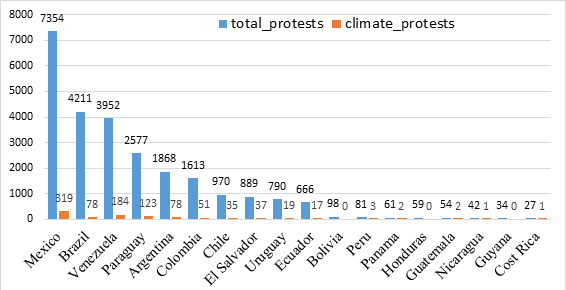
\includegraphics[width=3in,height=1.8in] {figures/climate/GSR_Climate_total.png}
		\label{fig:GSR_climate_number}
	}
	\subfigure[]{
		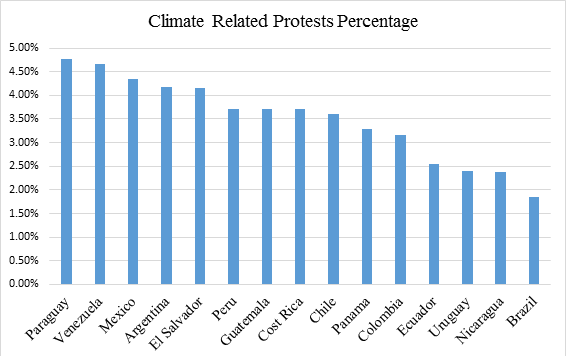
\includegraphics[width=3in,height=1.8in] {figures/climate/Climate_percentage.png}
		\label{fig:Climate_percentage}
	}	
	\caption{(a) GSR protest event distributions, (b) climate related protest percentage.}
\label{fig:total_climate}
\end{figure}

\begin{figure}[th]
	\centering
	\subfigure[]{
		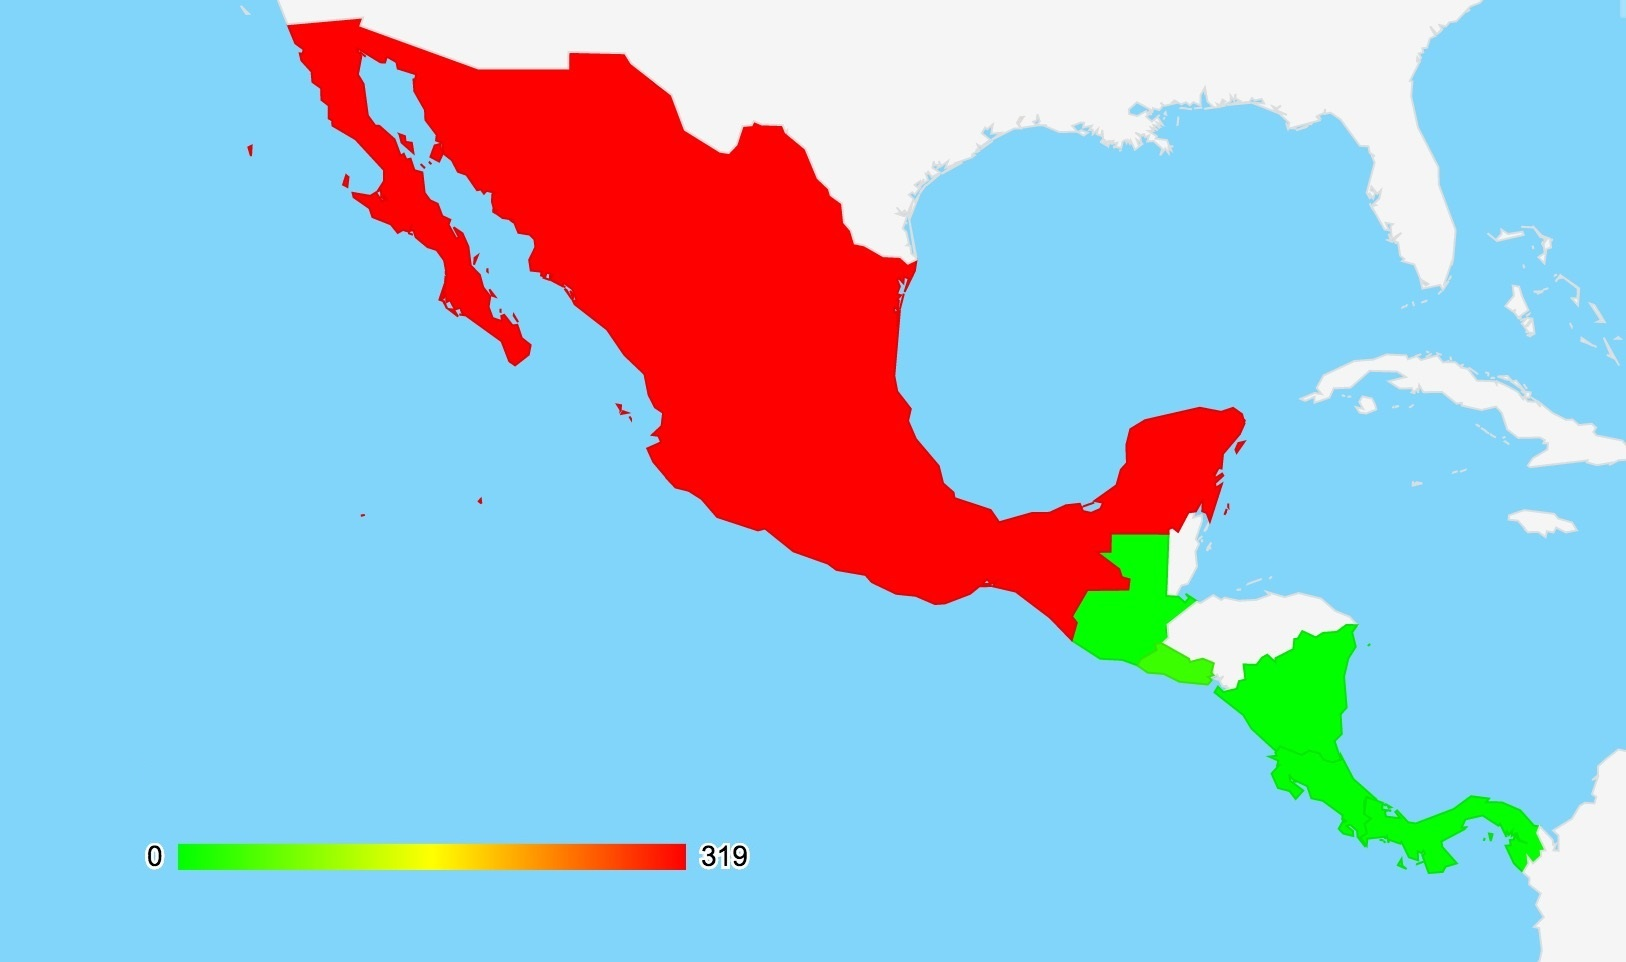
\includegraphics[width=2.8in] {figures/climate/WeatherProtest2.png}
		\label{fig:climate_weather_map2}
	}
	\subfigure[]{
		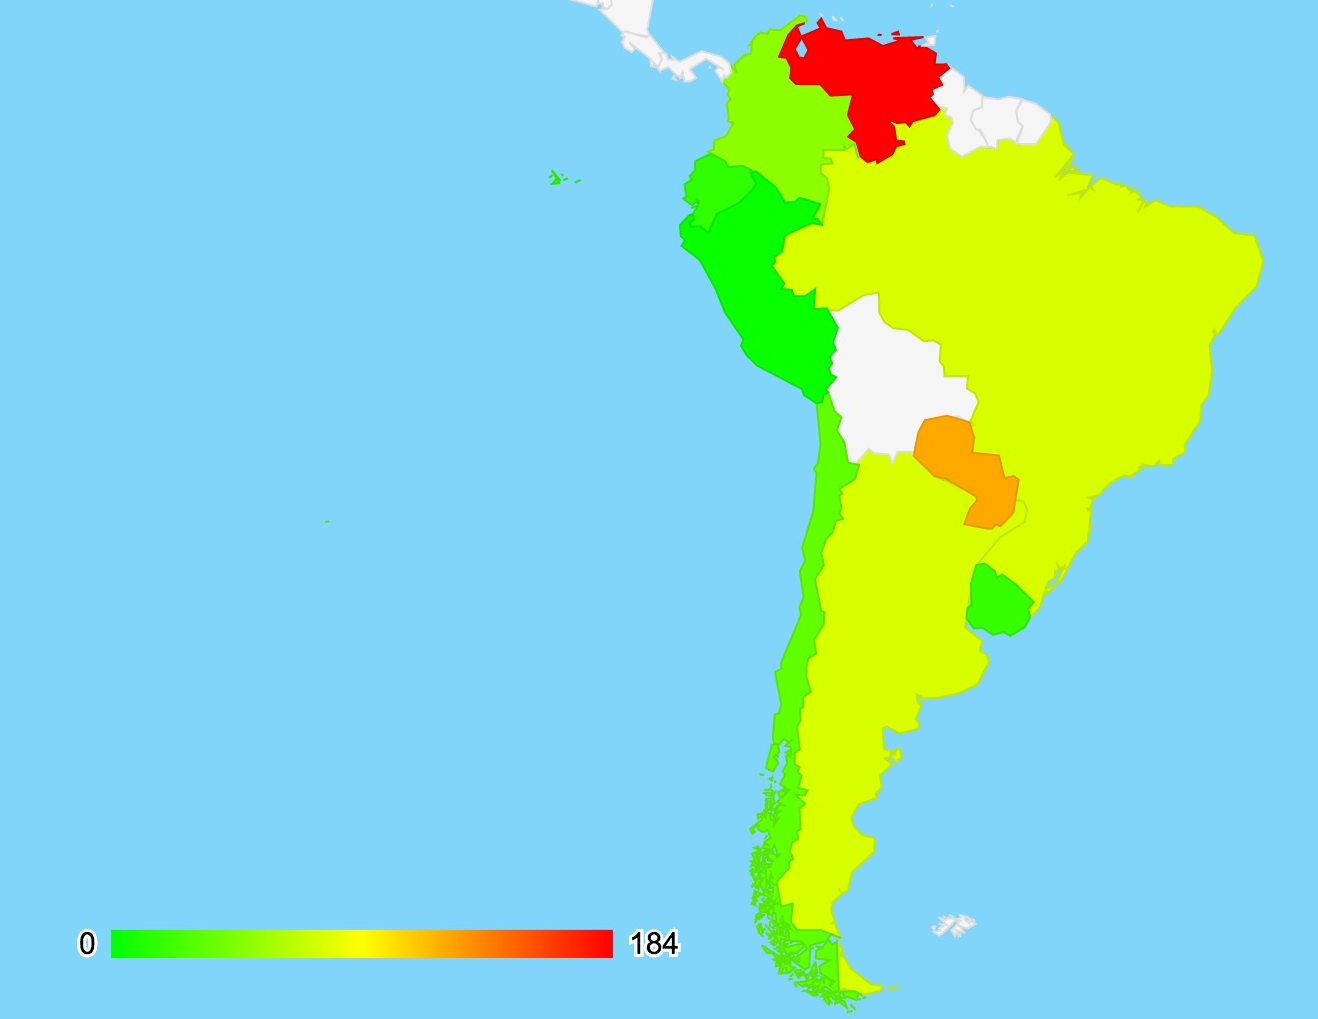
\includegraphics[width=2.8in] {figures/climate/WeatherProtest1.png}
		\label{fig:climate_weather_map1}
	}	
	\subfigure[]{
		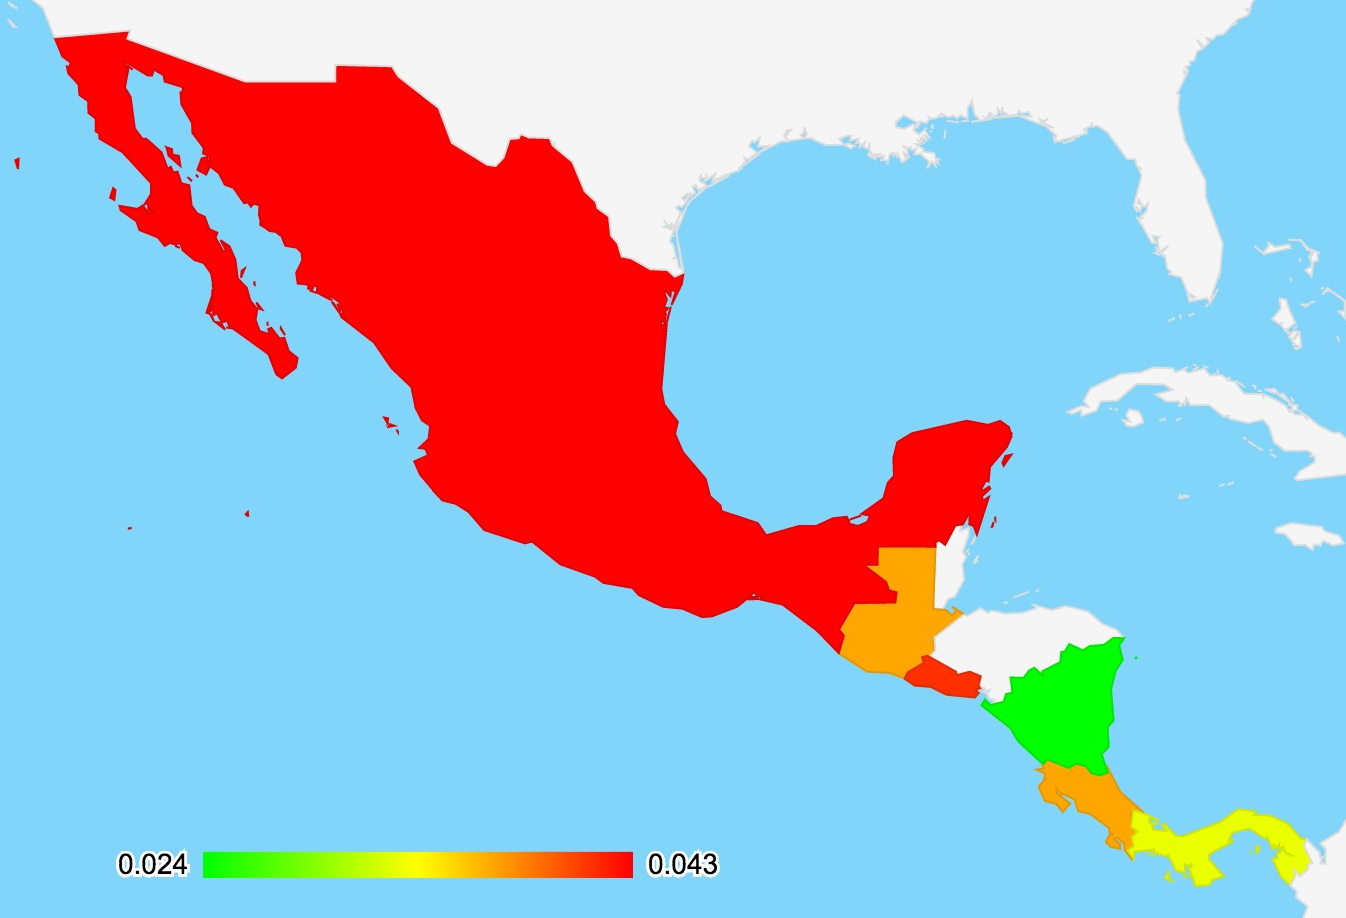
\includegraphics[width=2.8in] {figures/climate/Percentage2.png}
		\label{fig:GSR_Percentage2}
	}
	\subfigure[]{
		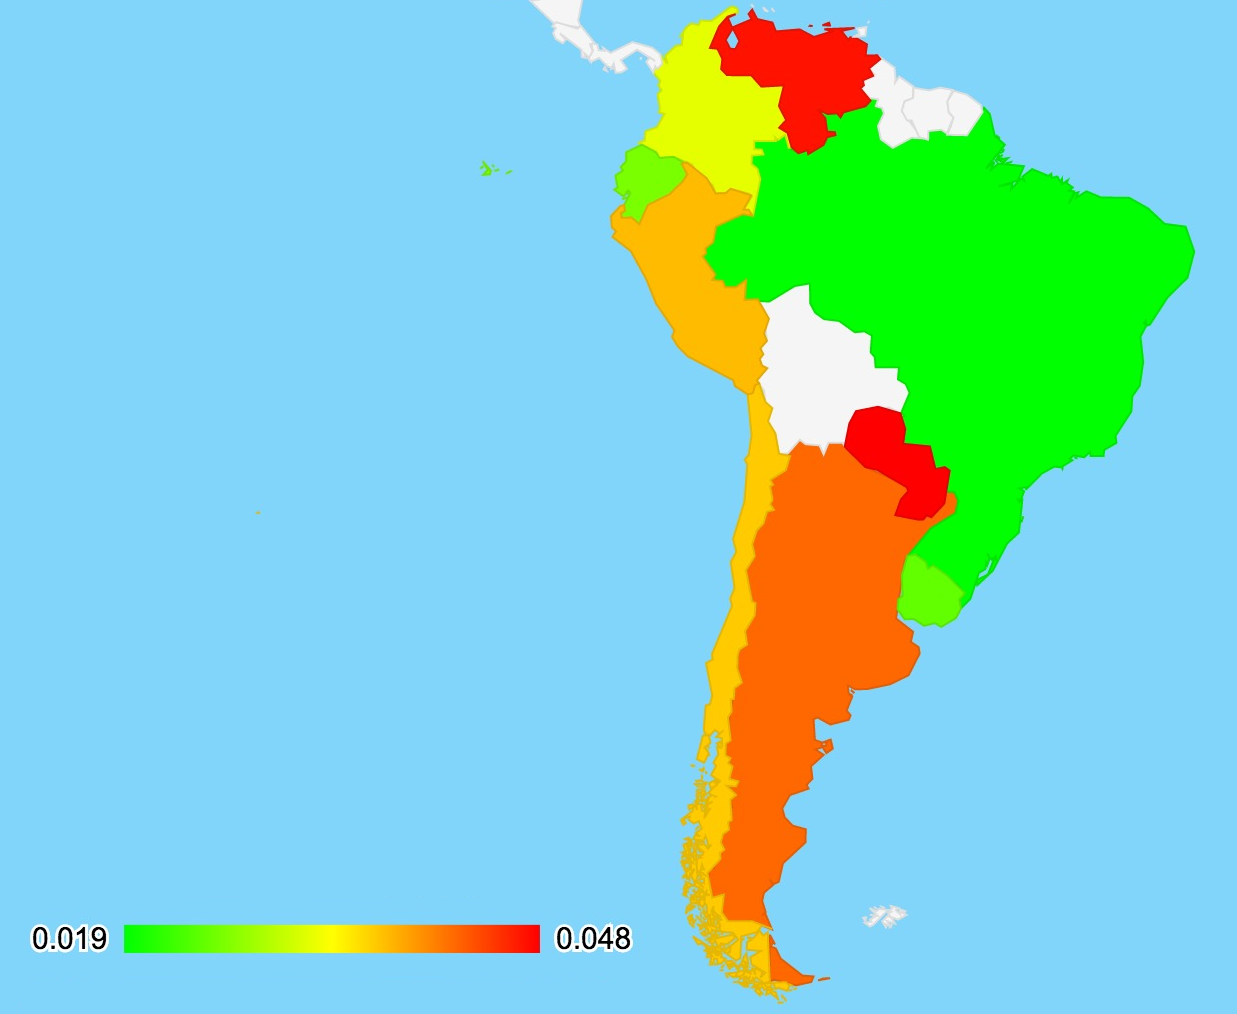
\includegraphics[width=2.8in] {figures/climate/Percentage1.png}
		\label{fig:Climate_Percentage1}
	}
	\caption{(a)(b) Climate protest events in South America. (c)(d) Climate protest percentage in South America.}
\label{fig:map_climate_no}
\end{figure}

%
%\begin{figure}[th]
%	\centering
%	\subfigure[]{
%		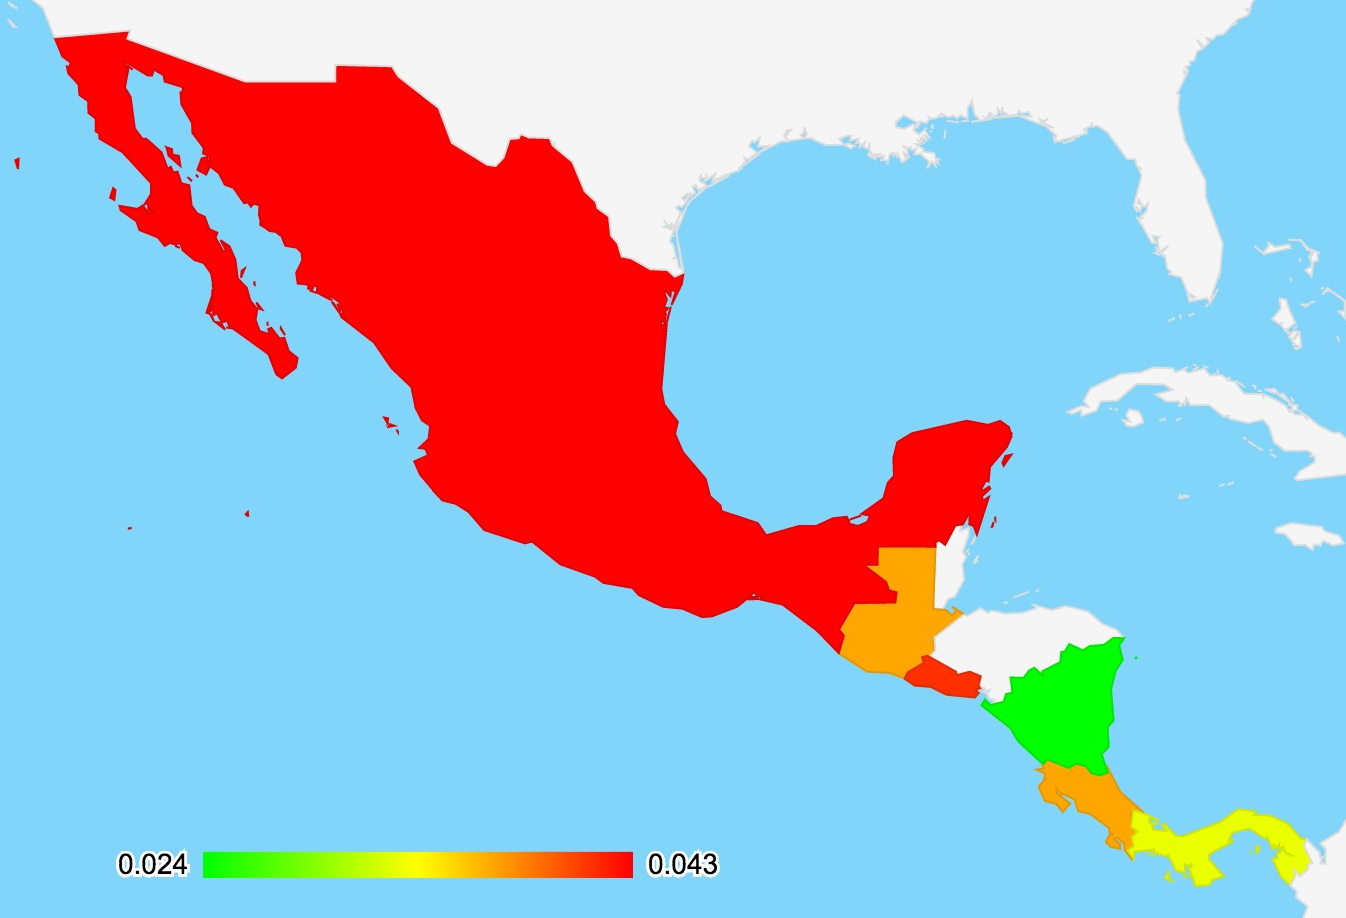
\includegraphics[width=2.8in] {figures/climate/Percentage2.png}
%		\label{fig:GSR_Percentage2}
%	}
%	\subfigure[]{
%		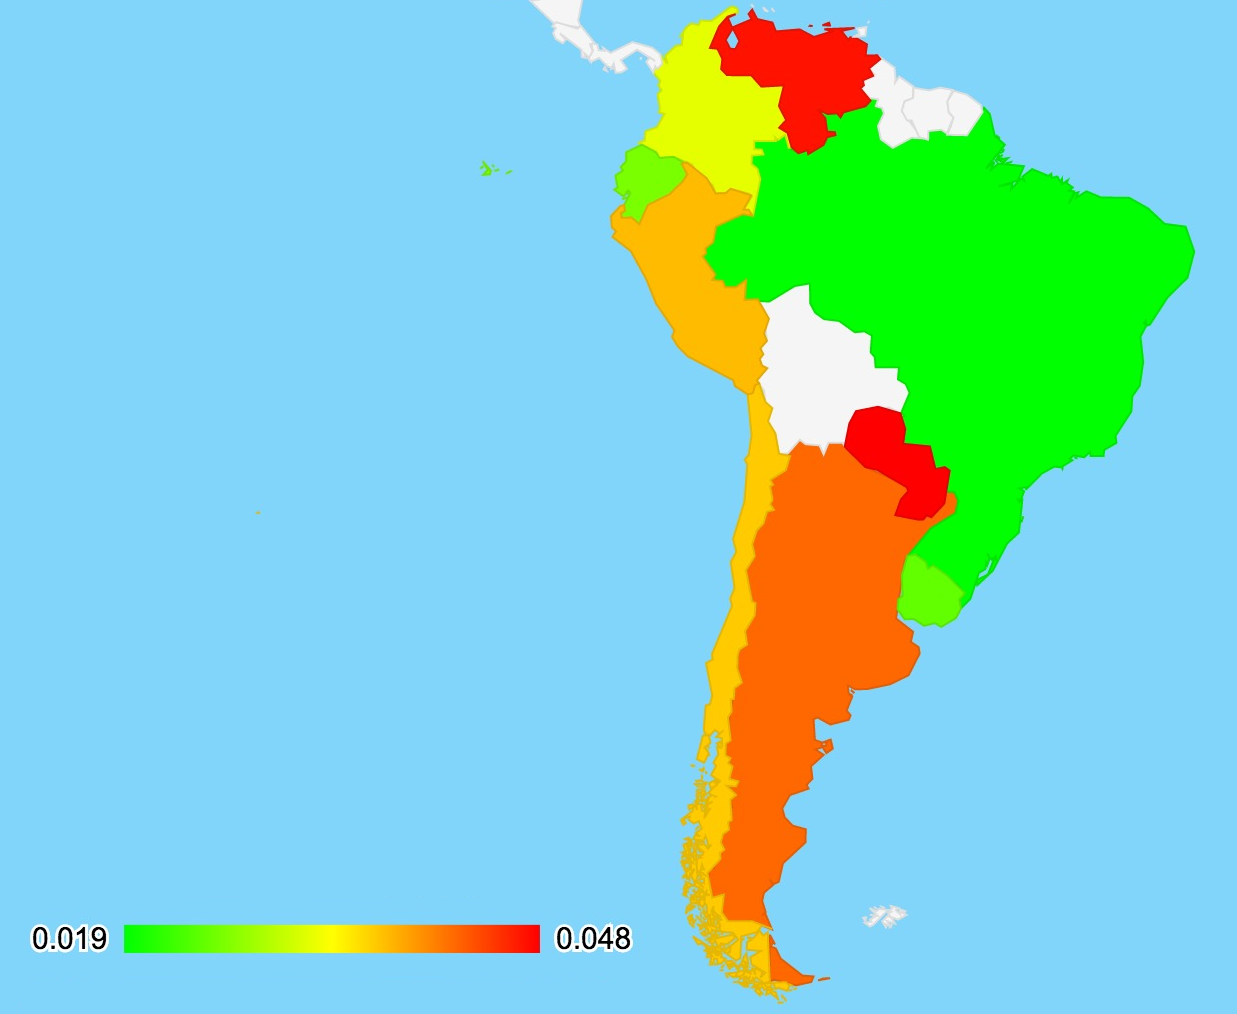
\includegraphics[width=2.8in] {figures/climate/Percentage1.png}
%		\label{fig:Climate_Percentage1}
%	}	
%	\caption{Climate protest percentage in South America.}
%\label{fig:map_percentage}
%\end{figure}

We study 25352 GSR events across South American counties from Jan, 2011 to March, 2015. Among all the 25352 GSR events, 974 events are classified into climate-related events, which is equal to 3.84\%. The GSR protest events and climate-related protests events for each country is plotted in Figure~\ref{fig:total_climate}. Mexico has both the largest GSR protest events and climate-related protest events. However, in terms of the percentages of the climate-related events, Paraguay is the highest (4.7\%) and Bolivia is the lowest (1\%). To have an overview of climate protests events distribution, we plot the climate protest events and its percentage over GSR in Figure~\ref{fig:map_climate_no}. It is important to evaluate how climate-related events has varied and changed in the past. We plot the monthly climate-related events and the percentages of climate-related protest events for each country in Figure~\ref{fig:climate_percentage}.




\begin{figure}[th]
	\centering
	\subfigure[]{
		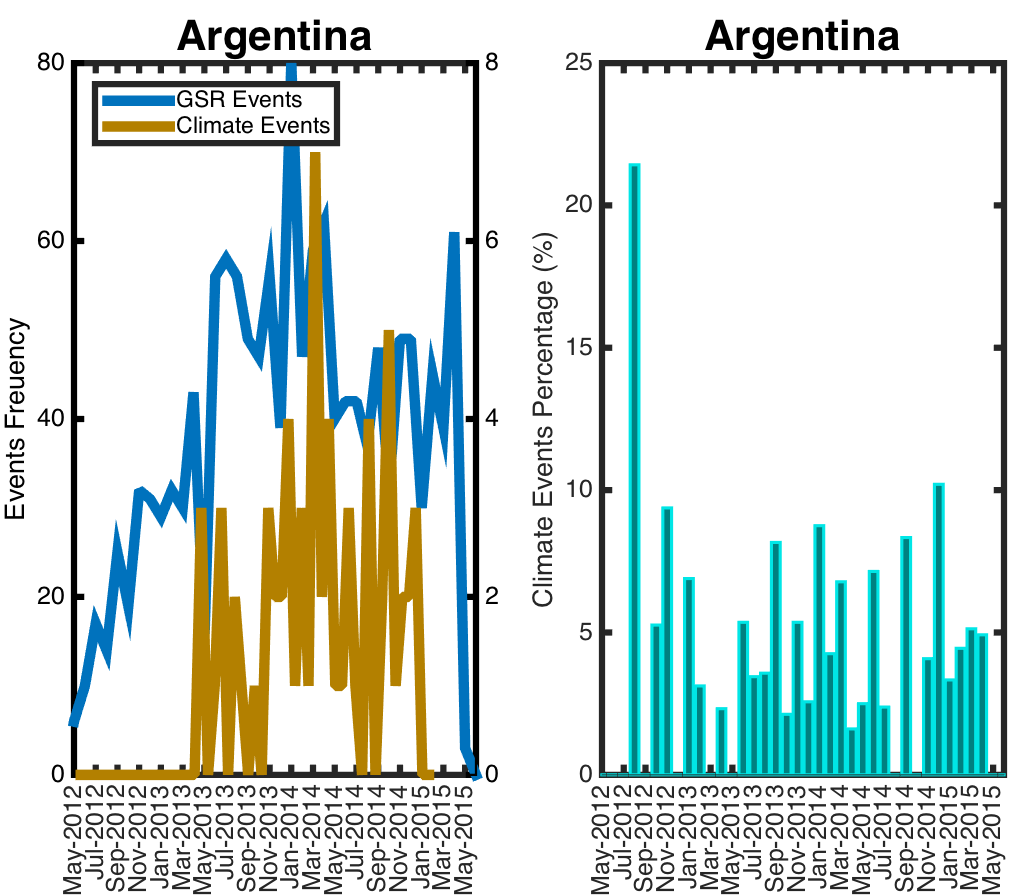
\includegraphics[width=3in,height=1.95in] {figures/climate/Argentina_percentage.png}
		\label{fig:percentage_Argentina}
	}
	\subfigure[]{
		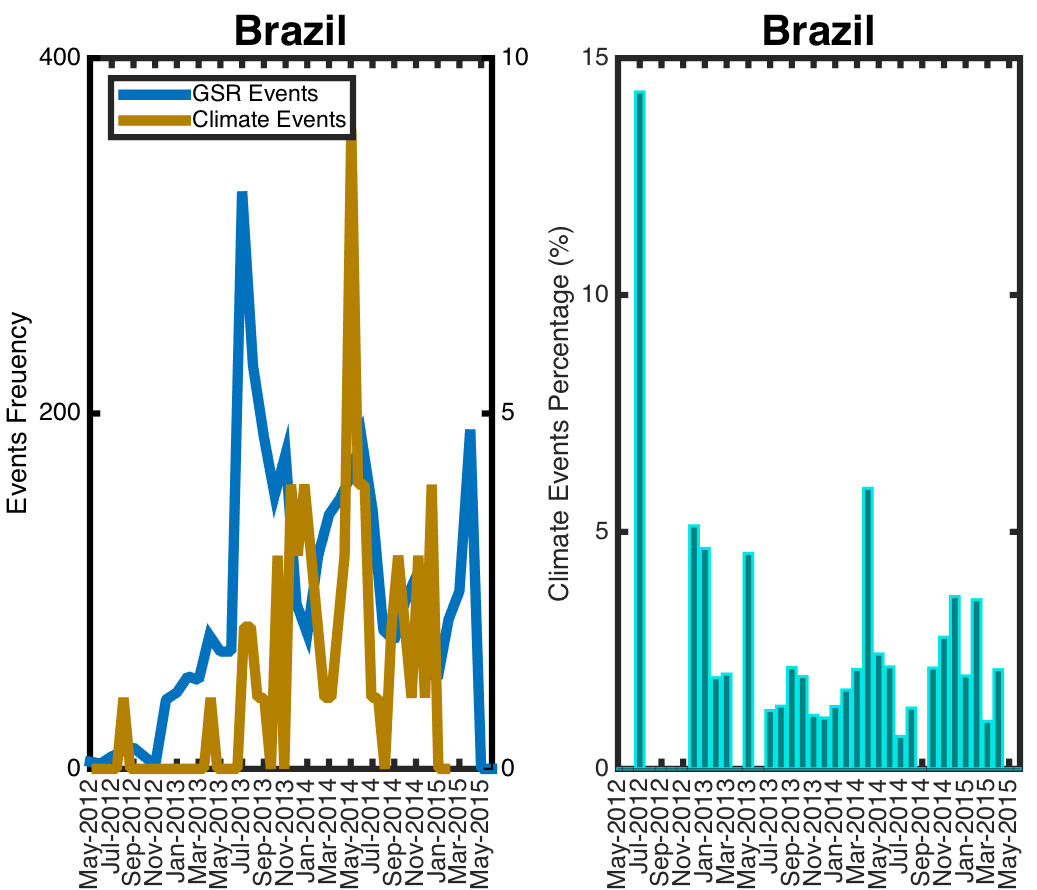
\includegraphics[width=3in,height=1.95in] {figures/climate/Brazil_percentage.png}
		\label{fig:percentage_Brazil}
	}	
	\subfigure[]{
		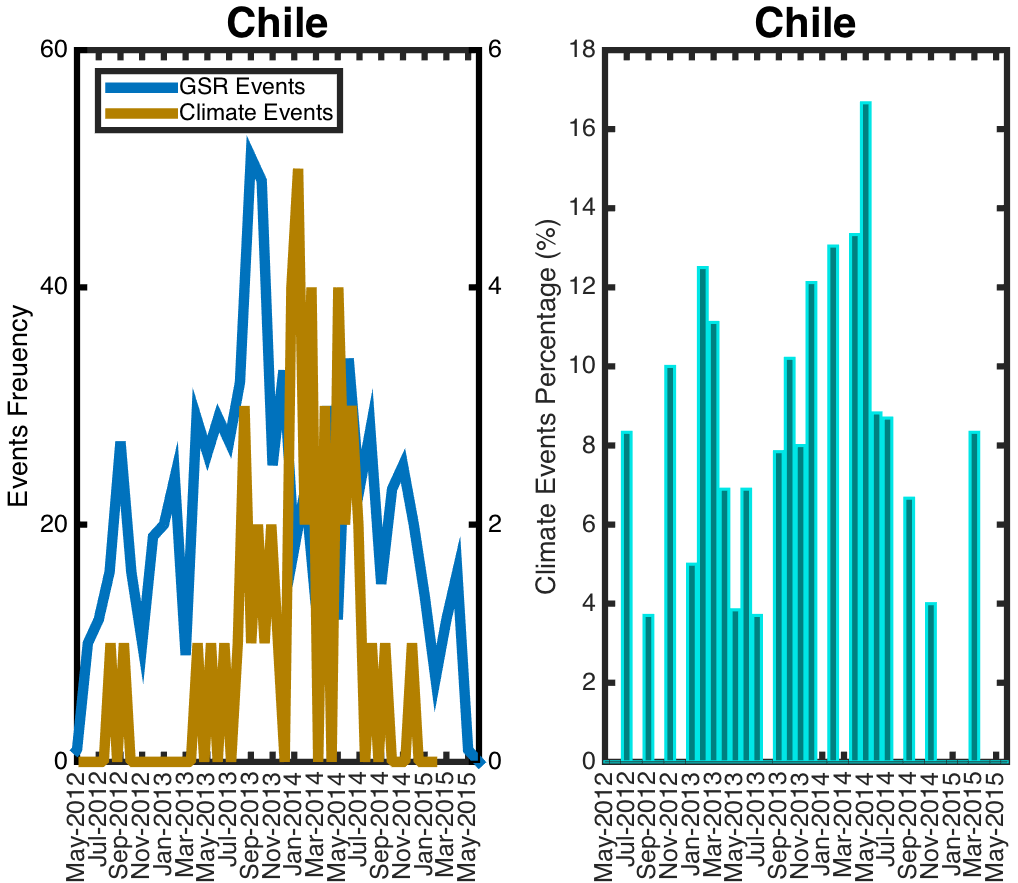
\includegraphics[width=3in,height=1.95in] {figures/climate/Chile_percentage.png}
		\label{fig:percentage_Chile}
	}
	\subfigure[]{
		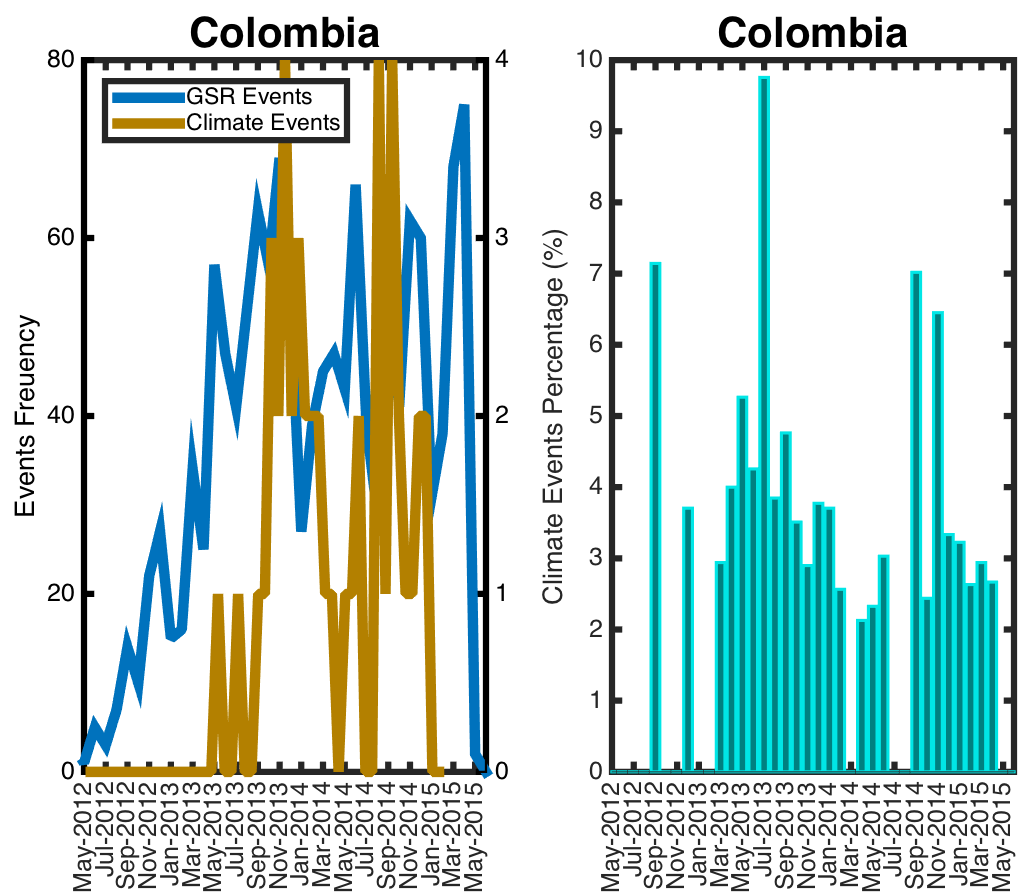
\includegraphics[width=3in,height=1.95in] {figures/climate/Colombia_percentage.png}
		\label{fig:percentage_Colombia}
	}
	\subfigure[]{
		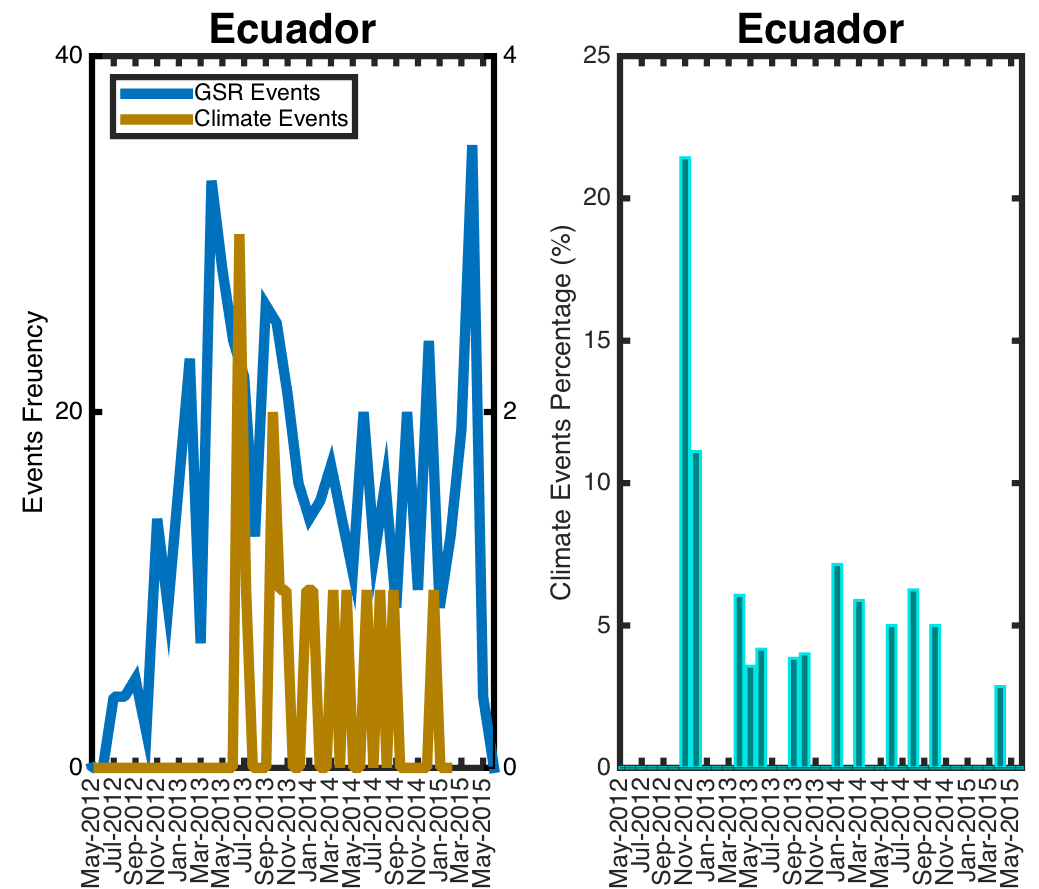
\includegraphics[width=3in,height=1.95in] {figures/climate/Ecuador_percentage.png}
		\label{fig:percentage_Ecuador}
	}
	\subfigure[]{
		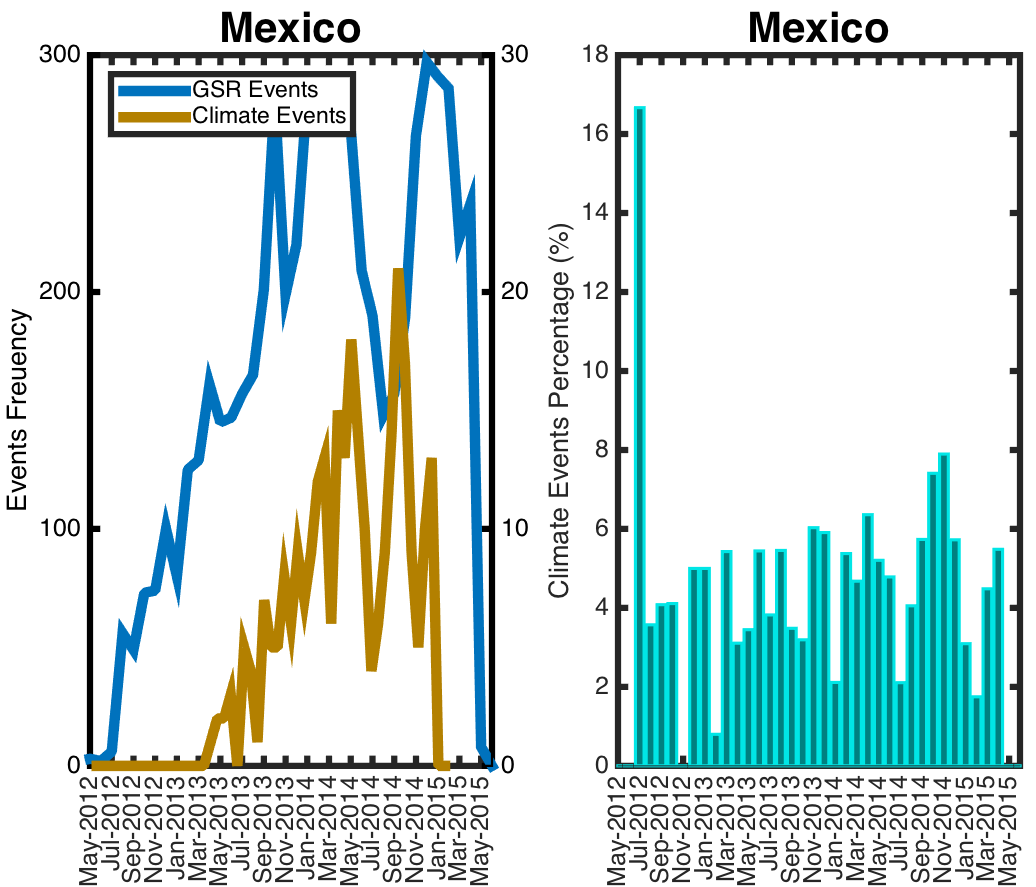
\includegraphics[width=3in,height=1.95in] {figures/climate/Mexico_percentage.png}
		\label{fig:percentage_Mexico}
	}
	\subfigure[]{
		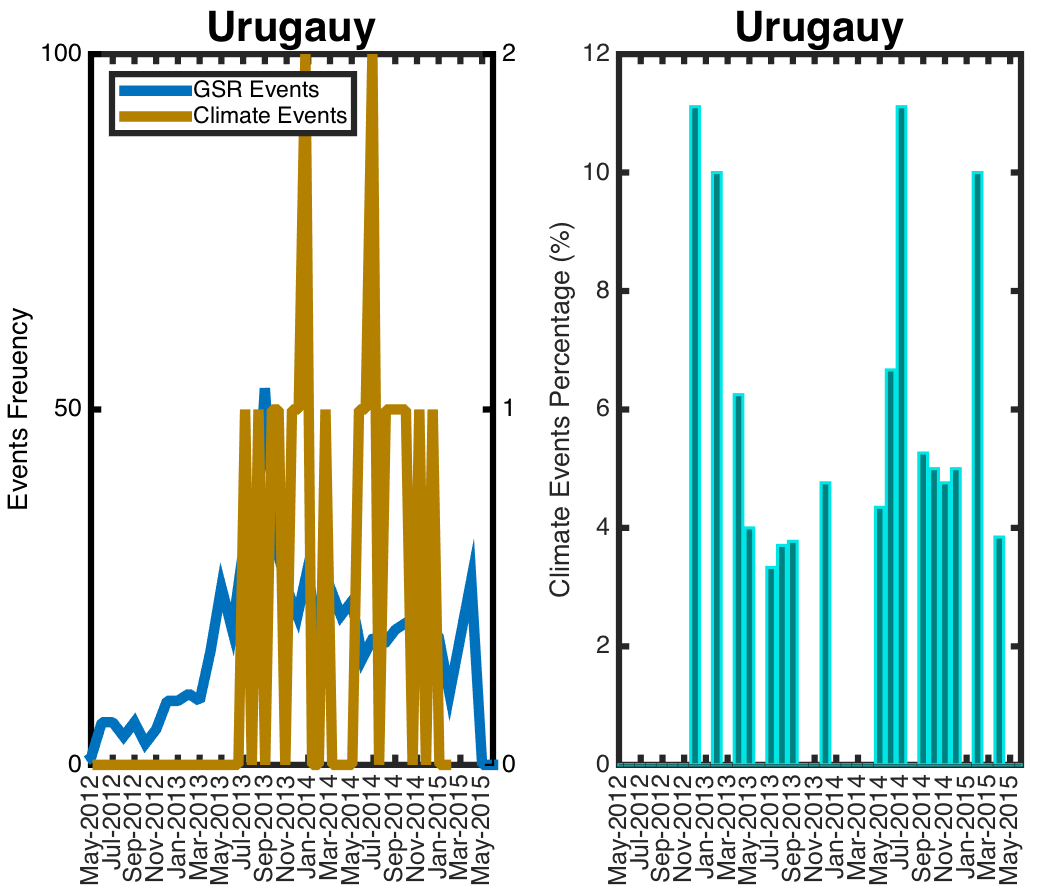
\includegraphics[width=3in,height=1.95in] {figures/climate/Urugauy_percentage.png}
		\label{fig:percentage_Urugauy}
	}
	\subfigure[]{
		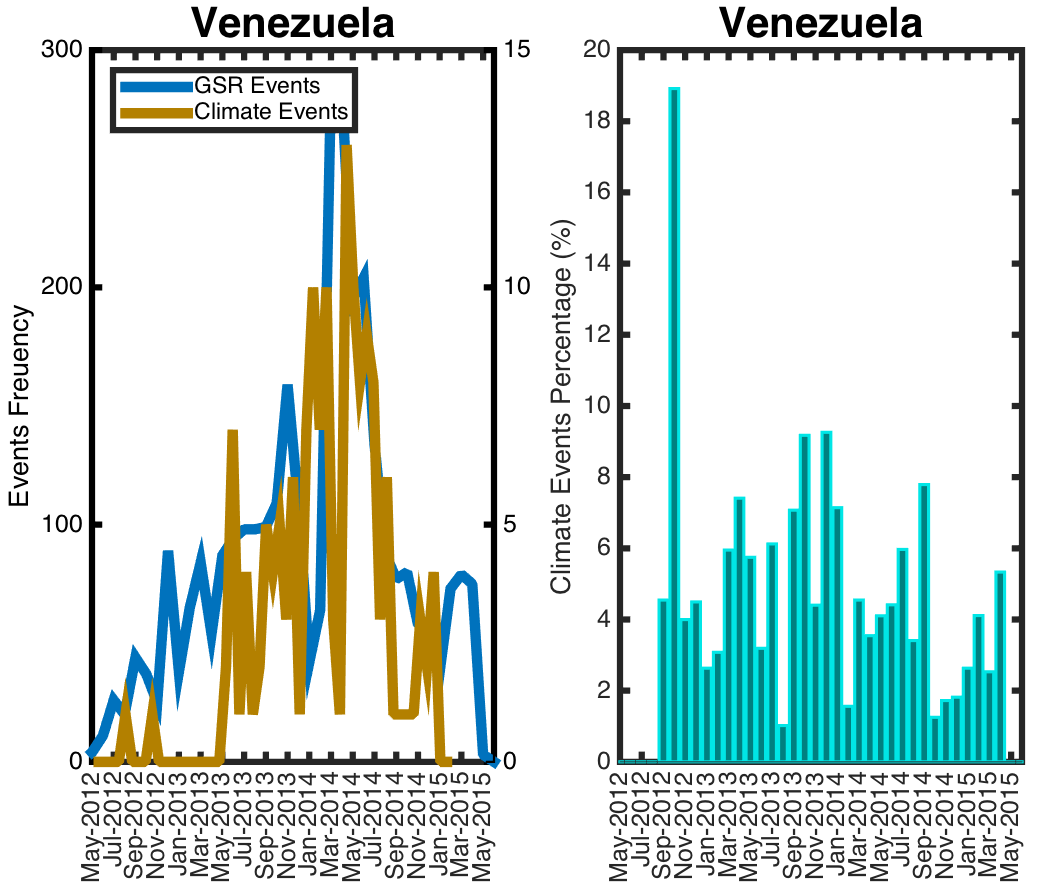
\includegraphics[width=3in,height=1.95in] {figures/climate/Venezuela_percentage.png}
		\label{fig:percentage_Venezuela}
	}
	\caption{Compare GSR events, climate events and climate events percentage of South American.}
\label{fig:climate_percentage}
\end{figure}



GSR event defines six different protest event types according to the concerns of people involved, they are employment, housing, energy \& resources, economic polices, other government policies, other. We are interested to see which event type is most dominant of all the climate related protest events. We plot the event type distributions for each country in Figure~\ref{fig:climate_eventType}.

%As we can see that even each county has different number of climate-related events, however, the distributions of event type are roughly the same, which means the type 011 has the highest percentages while type 016 the lowest.

\begin{figure}[t]
	\centering
	\subfigure[]{
		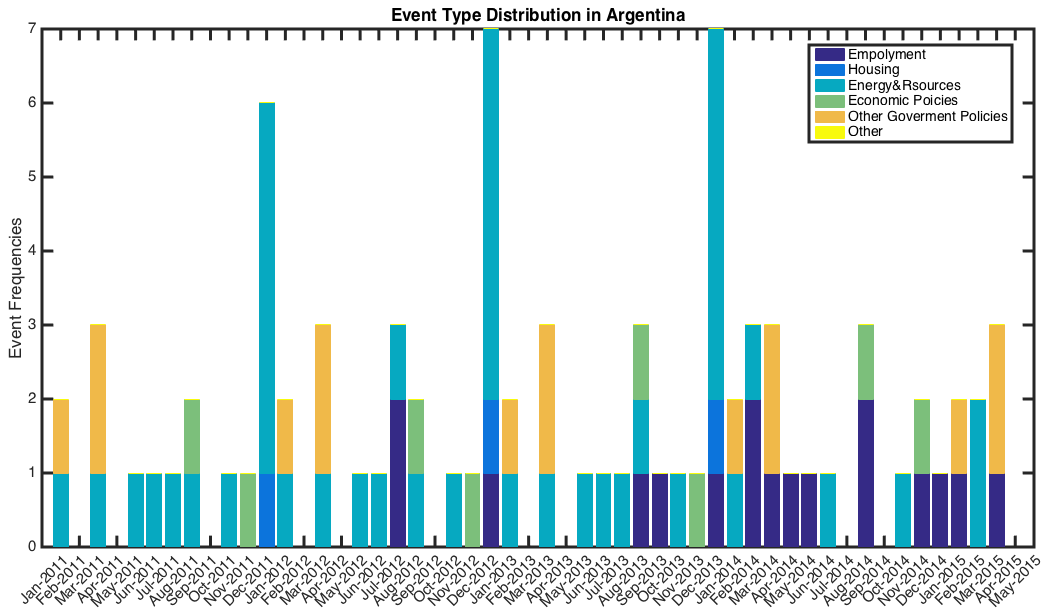
\includegraphics[width=3in,height=1.8in] {figures/climate/Argentina_type.png}
		\label{fig:type_Argentina}
	}
	\subfigure[]{
		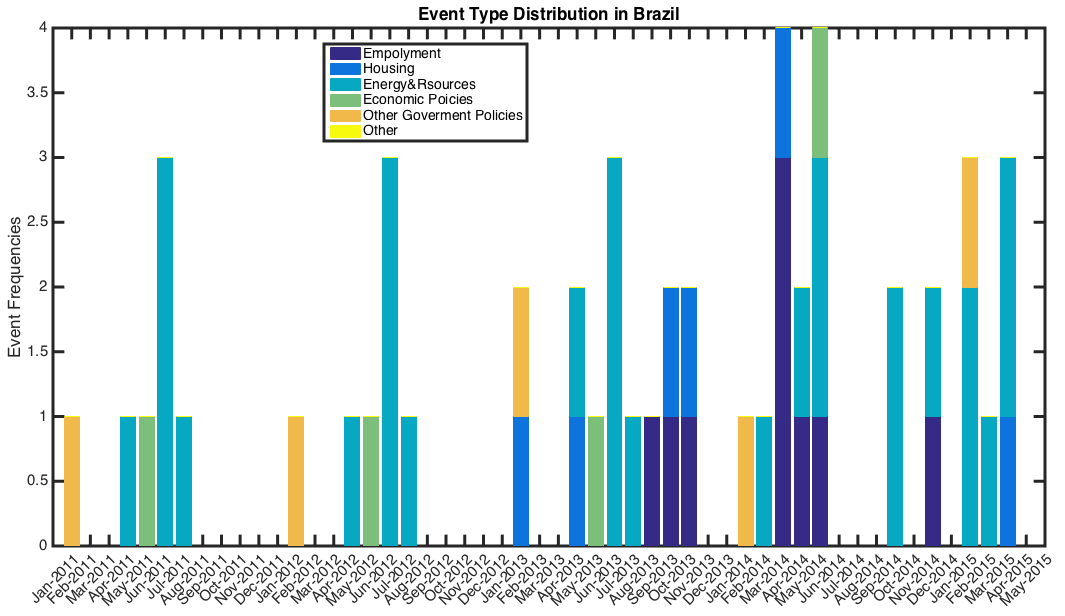
\includegraphics[width=3in,height=1.8in] {figures/climate/Brazil_type.png}
		\label{fig:type_Brazil}
	}	
	\subfigure[]{
		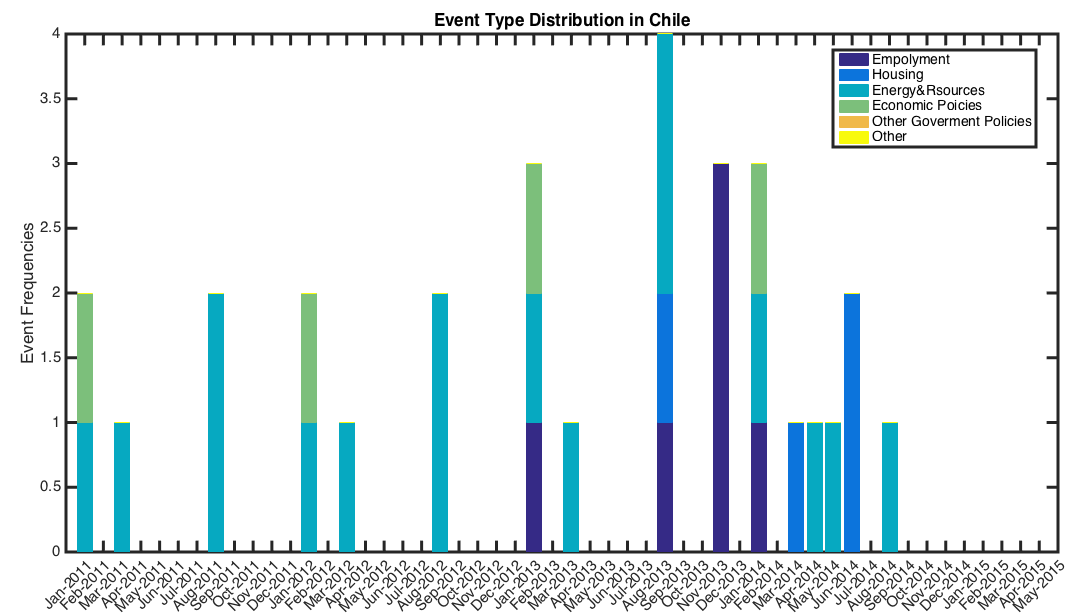
\includegraphics[width=3in,height=1.8in] {figures/climate/Chile_type.png}
		\label{fig:type_Chile}
	}
	\subfigure[]{
		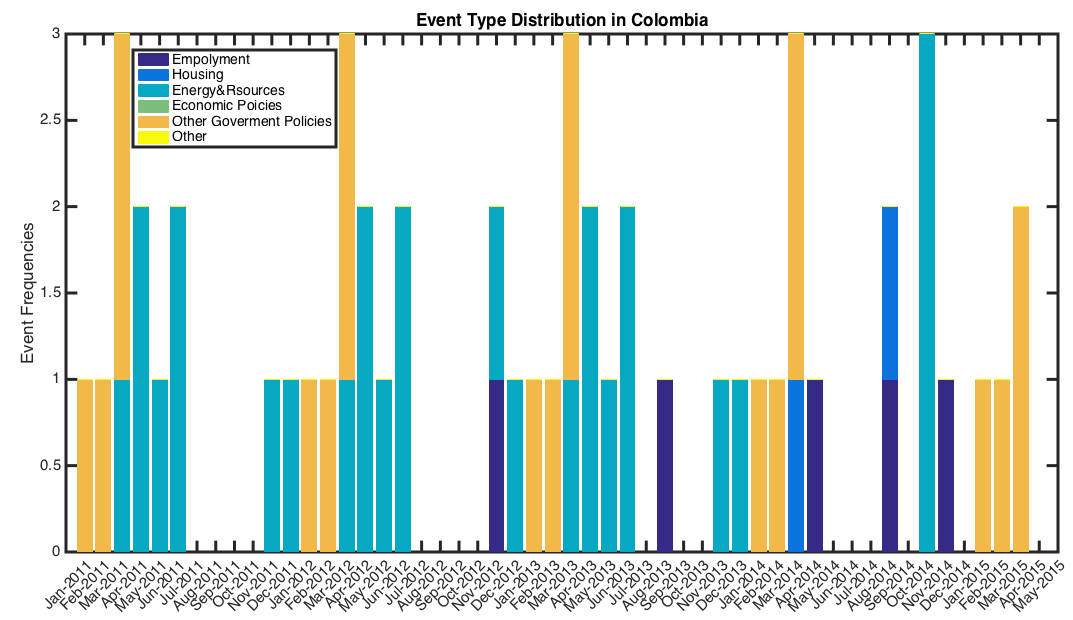
\includegraphics[width=3in,height=1.8in] {figures/climate/Colombia_type.png}
		\label{fig:type_Colombia}
	}
	\subfigure[]{
		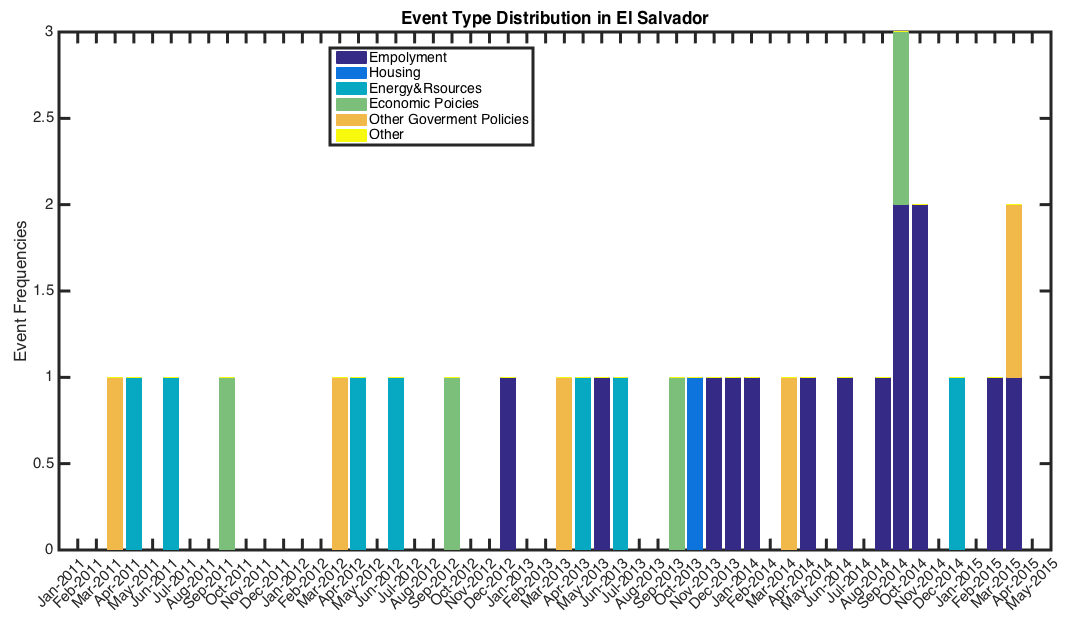
\includegraphics[width=3in,height=1.8in] {figures/climate/Elsd_type.png}
		\label{fig:type_Elsd}
	}
	\subfigure[]{
		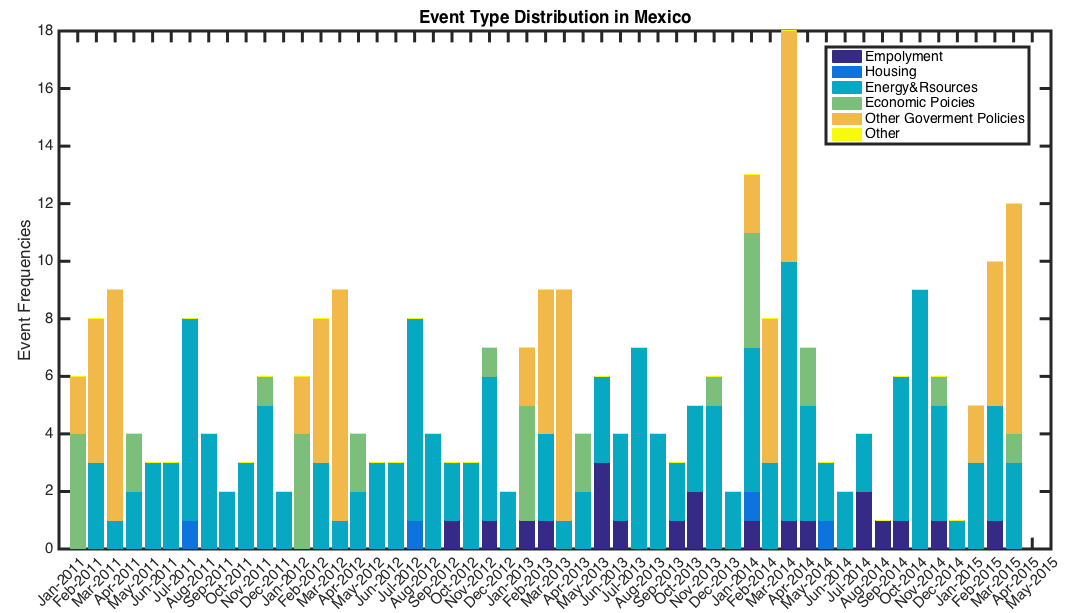
\includegraphics[width=3in,height=1.8in] {figures/climate/Mexico_type.png}
		\label{fig:type_Mexico}
	}
	\subfigure[]{
		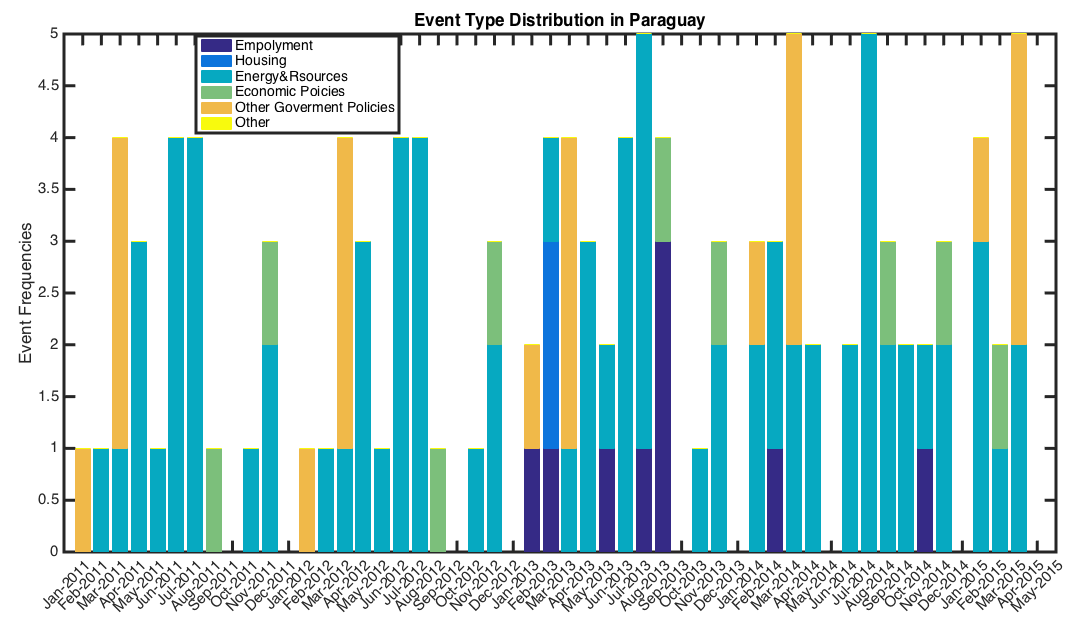
\includegraphics[width=3in,height=1.8in] {figures/climate/Paraguay_type.png}
		\label{fig:type_Paraguay}
	}
	\subfigure[]{
		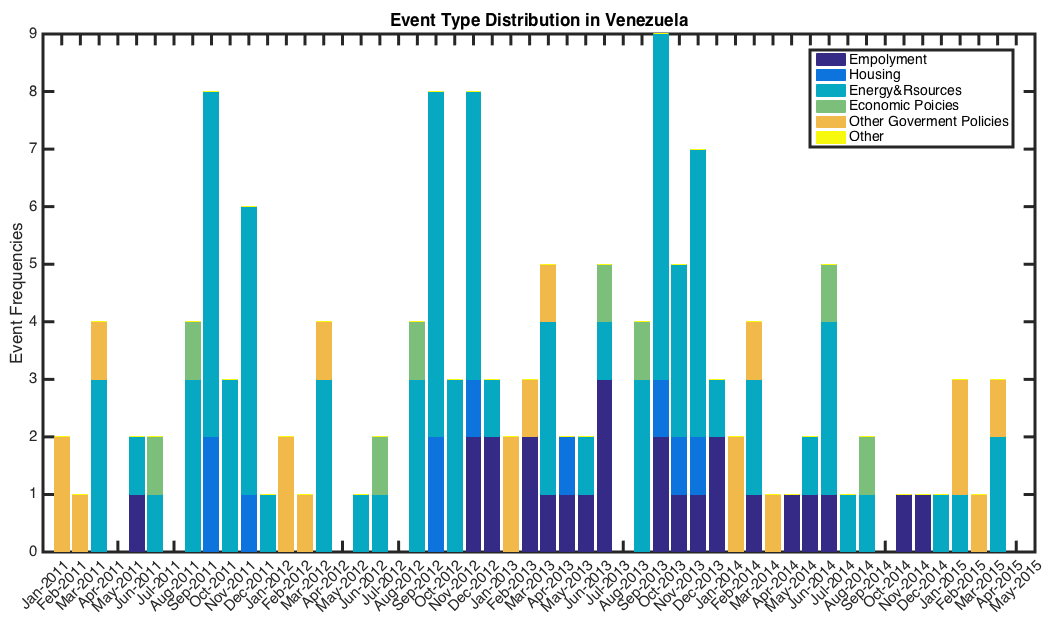
\includegraphics[width=3in,height=1.8in] {figures/climate/Venezuela_type.png}
		\label{fig:type_Venezuela}
	}
	\caption{Event type distribution of climate events for South American.}
\label{fig:climate_eventType}
\end{figure}

\subsection{Information Chain}
The story telling algorithm we employed is based on weighted scores of similarities across news articles for three sets of features: textual features (related to keywords), spatial features (such as locations and geographical coordinates), and actors (such as person(s), and organizations mentioned in the articles)~\cite{ninguncovering}. The chaining methodology is developed with the goal of identifying all documents related to a climate change story and to keep track of the news story as new documents arrive. Documents belonging to such a chain cover the same event and are ordered by time. The algorithm operates in an incremental fashion wherein every new input article is analyzed as it arrives and is appended to already existing chain(s). This analysis involves a two-step process. In the first step, we compare an incoming article Di to articles from the last n1 days to identify the most similar articles and then designate candidate chains to which the current article can be attached to. If no similar articles are found, then a new chain is created with this article as a seed.
Further, to assess if two documents are referring to the same underlying context, we calculate their similarity scores with respect to three features:
- textual features,
- spatial features, and
- actors.

The storytelling algorithm is employed to track the evolvement process of a climate event, from its beginning to its ending, and finally develop into a civil unrest event. To avoid confusion, we build story chains country by country. We collect each country�s RSS news from its top leading news agencies, for instance, Brazil news comes from Brazil� O Globo, Estadao, and Jornal do Brasil. In addition to this data, we also have access to a human curated list of civil unrest events that happened during this period. This list, called the Gold Standard Report (GSR) described in~\cite{ramakrishnan2014beating}, contains news reports for each event from the three major news sources. For each country�s document stream, we employ storytelling algorithm. The following shows some story chains for climate related protest events.

\begin{figure}[th]
	\centering
	\subfigure[]{
		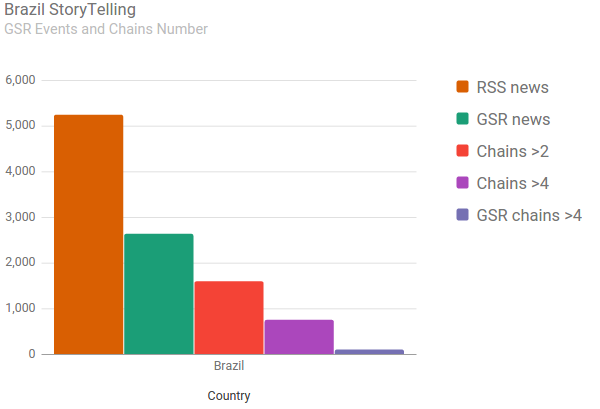
\includegraphics[width=3in,height=2.1in] {figures/climate/Brazil_story_bar.png}
		\label{fig:Brazil_story1}
	}
	\subfigure[]{
		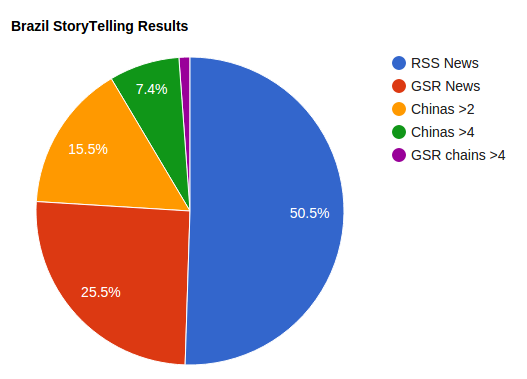
\includegraphics[width=3in,height=2.1in] {figures/climate/Brazil_story_pie.png}
		\label{fig:Brazil_story2}
	}	
	\caption{Story chain overview of Brazil protests events.}
\label{fig:Brazil_storytelling}
\end{figure}



\begin{figure}[th]
	\centering
	\subfigure[]{
		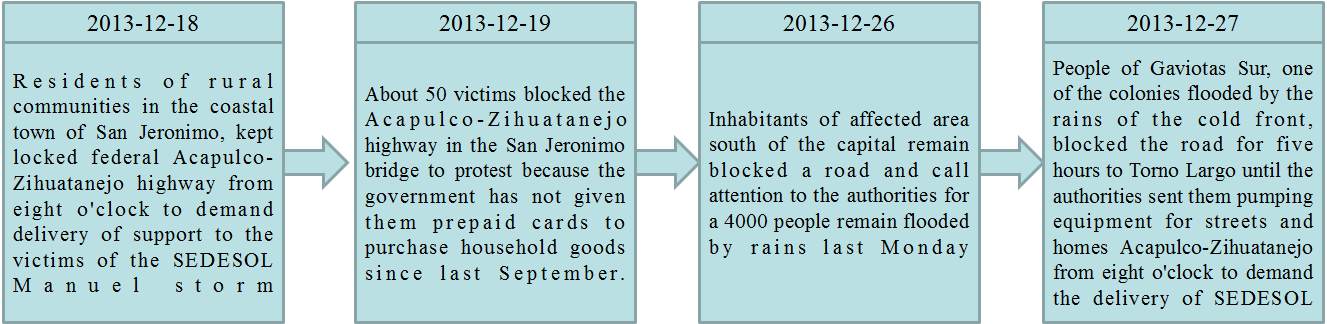
\includegraphics[width=5in,height=1.5in] {figures/climate/Mexico_hurricane.png}
		\label{fig:Mexico_story}
	}
	\subfigure[]{
		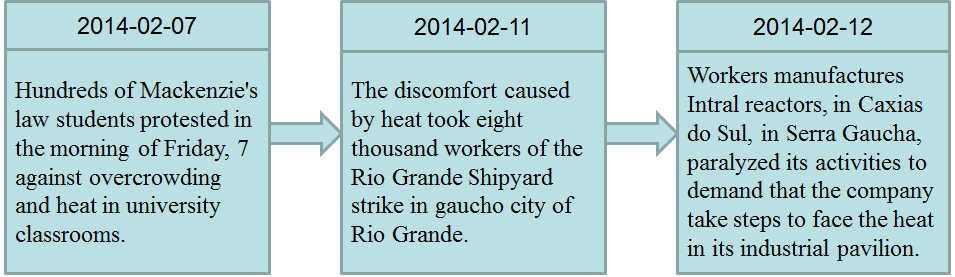
\includegraphics[width=5in,height=1.3in] {figures/climate/Brazil_heat.png}
		\label{fig:Brazil_story}
	}	
	\subfigure[]{
		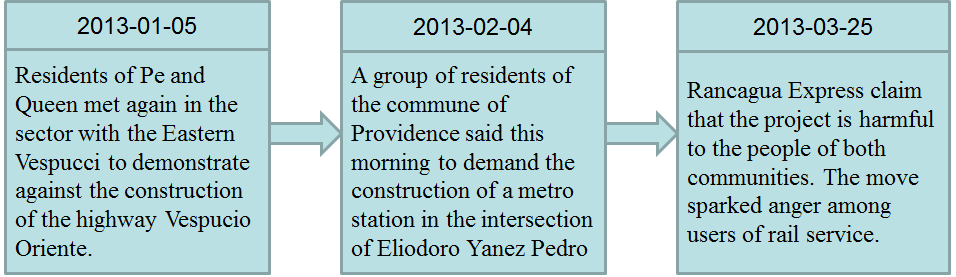
\includegraphics[width=5in,height=1.3in] {figures/climate/Chile-construction.png}
		\label{fig:Chile_story}
	}	
	\caption{Story chain for (a) Mexico hurricane climate events. (b) Brazil heat wave events. (c) Chile anti-construction events.}
\label{fig:storytelling}
\end{figure}



%\subsection{Dynamic Flow in Twitter}



%We know climate changes can cause health, economic problems, but will that effect the society stabilization, if so, how large extent?
%
%Create a database of climate change extreme weather keywords. We can also use DQE to generate more keywords, in Spanish and Portuguese.
%Filter the GSR descriptions, see how many GSR events talking about climate related words, what are their categories.
%
%Different countries civil unrest may be influenced under different climate change scenarios.
%
%Find the evidence for climate influence civil unrest
%Run storytelling
%
%
%There is a problem, given initial keywords, the DQE will capture protests which are non-climate related protests. Shall we filter those non-climate protests or keep it? Thanks!
%
%1. improve storytelling procedure, get more interesting results
%2. cluster DQE based on spatial information, to show DQE word cloud results (drought, storm) at different locations.
%3. build filter / classifier, to get the precise climate protests events in each country
%4. start to write the climate chapter, because visualization like map plotting also takes a lot of time.

\section{Future Work Time Table}
The proposed work is going to carry out according to time table shown on Figure~\ref{fig:timetable}.

\begin{figure}[h]
\centering
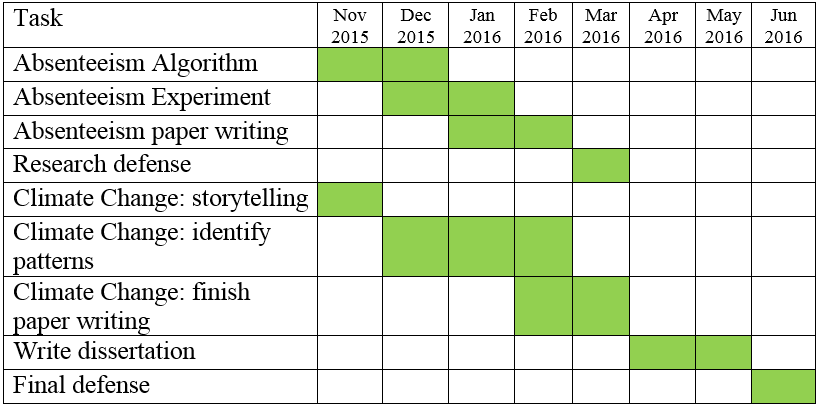
\includegraphics[height=2in]{figures/timetable.png}
\caption{Future work time table.}
\label{fig:timetable}
\end{figure}

\endgroup
